\chapter{Graph analysis}
This chapter performs a final analysis on antibiotic patterns through a graph database, applying graph algorithms to identify similarities between prescriptions and popularity among prescriptions. Results are then compared with $k$-means clustering.

\section{Graph databases}
\textbf{Graph databases} are data management systems allowing persistent representation of entity and relationship in a graph structure, implementing the \textit{Property Graph Model} efficiently down to the storage level.

A \textbf{graph} $G\: =\: <E, V>$ is an abstract data type showing connections (edges $E$) between pairs of vertices ($V$). Nodes identify entities and their properties, while relationships are joining attributes between tables with eventual additional characteristics. 

Unlike other databases, \textit{relationships take first priority}. A graph database is purpose-built to handle highly connected data, providing great performance, flexibility and frictionless development.

Queries allow to match pattern of nodes and relationships in a graph, providing ACID transaction compliance without specifying details on how to implement operations. Graph-crossing and related algorithms are highly efficient.

\subsection{An overview on Neo4j}
Neo4j is an online graph database management system with Create, Read, Update and Delete (CRUD) operations working on a graph data model. The data model for a graph database is also significantly simpler and more expressive than those of relational or other NoSQL databases.

In Neo4j, everything is stored in the form of an \textbf{edge}, \textbf{node}, or \textbf{attribute}. Each node and edge can have any number of attributes, and both nodes and edges can be labelled. Labels can be used to narrow searches, improving speed.

Queries are written using \textbf{Cypher}, a declarative graph query language that allows for expressive and efficient querying and updating of the graph. 

Cypher is inspired by a number of different approaches and builds on established practices for expressive querying, with SQL-inspired keywords and high-level semantics\cite{neo4jbook}.

\section{Prescription coupling}
An excessive usage of antibiotics causes death of microorganisms in the human body which provide to maintaining immune cells and killing certain oral infections\cite{bacteria}.

To equilibrate the intestinal flora, lactic ferments are often taken together with antibiotics, so that new ``good'' bacteria can restore the probiotic action.

If this hypothesis is correct, the dataset will show antibiotic prescriptions \textbf{paired with other drugs}, on the same date --- or it will highlight potential linkings between infections and other pathologies receiving a specific prescription.

\section{Goals}
Goals of analytics through graphs is completion of antibiotic patterns changes and patient journey, providing a different point of view on those two important aspects altogether.

This part of the research aims to focus on:
\begin{itemize}
	\item Co-prescriptions, understanding whether specified couples of drugs are often prescribed together;
	\item Clustering in communities, to identify similar kinds of doctors according to their prescription history;
	\item Centrality measures of nodes, to highlight particularly important entities in the graph.
\end{itemize}

\section{Practical approach}

\subsection{Relational database structure}
The available data comprehends patients, general practitioners, and their prescriptions in the time span from 2000 to 2018, located in Campania. Summarising the amount of records for each entity:
\begin{itemize}
	\item 888 219 patients;
	\item 2 486 doctors;
	\item 118 716 403 prescriptions;
	\item 33 523 drugs.
\end{itemize}

Due to the amount and veracity of data, identifying a subset of records is useful to have detailed and targeted results, removing dispersive information and leaving a restricted pool of prescriptions, setting acceptability conditions. 

Since analytics are aimed to identify \textbf{antibiotic prescription patterns}, similarly to past approaches, a new dataset has been extracted, imposing the following constraints:
\begin{enumerate}
	\item AIC corresponding to an antibiotic;
	\item Prescription date between 2008-01-01 and 2017-12-31;
	\item Active general practitioners;
	\item Patients with usable information about gender, date of birth and location.
\end{enumerate}

This leads to obtaining a new model, composed by:
\begin{itemize}
	\item 670 634 patients;
	\item 1 377 doctors;
	\item 8 386 057 prescriptions;
	\item 2 802 antibiotics.
\end{itemize}

To allow analytics on patient journey and co-prescriptions, it is necessary to access all the prescriptions assigned to all patients belonging in the subset. A major extraction is performed from the main table, comprehending:
\begin{enumerate}
	\item Identifier of patients who received at least one antibiotic prescription \textbf{on the same date} as a generic prescription;
	\item Prescription date between 2008-01-01 and 2017-12-31.
\end{enumerate}

This reduces the number of other prescriptions, adding drugs not belonging to the antibiotic class. Duplicates, mistakes and empty fields are removed. 

Information loss is displayed in the figure below:
\begin{figure}[h]
	\centering
	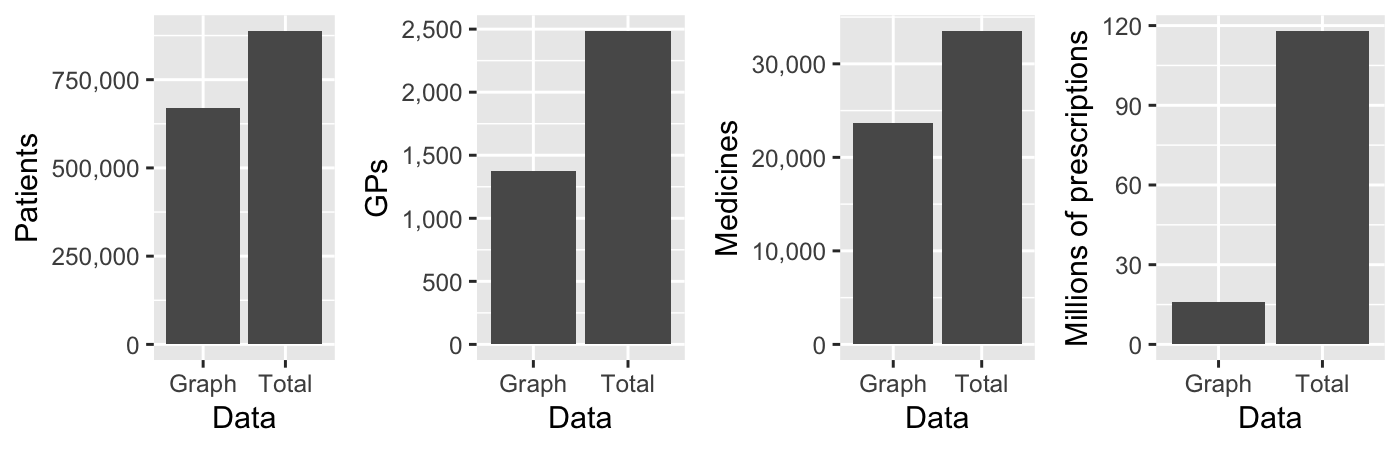
\includegraphics[scale=0.33]{../plots/graph-barplots.png}
	\caption{\small Information loss barplot}
\end{figure}

Values of prescriptions and medicines are aggregated in the plot, including both antibiotics and other drugs. The amount of removed prescriptions is most likely caused by the strict constraint of couples having the same date.

The resulting structure is an unweighted directed graph, with a data composition of:
\begin{itemize}
	\item 670 634 patients;
	\item 1 377 doctors;
	\item 8 328 272 prescriptions of antibiotics;
	\item 2 465 antibiotics;
	\item 7 587 009 other prescriptions;
	\item 21 248 other medicines.
\end{itemize}

\subsection{Migration of the database and graph modelling}
The database has to be structured following the SQL to Cypher practices and guidelines, assigning nodes and relationships in an appropriate way considering the existing dataset and the related goals. The entity-relationship model translates with the following nodes and attributes:
\begin{itemize}
	\item Patient;
	\begin{itemize}
		\item ID, birthdate, gender;
	\end{itemize}
	\item Doctor;
	\begin{itemize}
		\item ID; 
	\end{itemize}
	\item Antibiotic;
	\begin{itemize}
		\item AIC code, ATC code;
	\end{itemize}
	\item Medicine (anything not Antibiotic);
	\begin{itemize}
		\item AIC code, ATC code;
	\end{itemize}
	\item Prescription;
	\begin{itemize}
		\item patient, doctor, date, drug;
	\end{itemize}
	\item OtherPrescription (not Antibiotic Prescription);
	\begin{itemize}
		\item patient, doctor, date, drug.
	\end{itemize}
\end{itemize}

All nodes are imported, and main indexes are created for optimisation of queries speed. Relationships are then created according to IDs and AIC codes:
\begin{itemize}
	\item Prescription $-$ TO $\rightarrow$ Patient;
	\item Prescription $-$ FROM $\rightarrow$ Doctor;
	\item Prescription $-$ OF $\rightarrow$ Antibiotic;
	\item OtherPrescription $-$ TO $\rightarrow$ Patient;
	\item OtherPrescription $-$ FROM $\rightarrow$ Doctor;
	\item OtherPrescription $-$ OF $\rightarrow$ Medicine.
\end{itemize}

\section{Visualisation and analytics}
\subsection{Sample graph}
A sample graph is obtained using the \texttt{apoc} functions.

\begin{figure}[h]
	\centering
	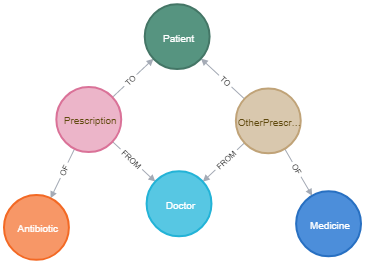
\includegraphics[scale=0.5]{./images/sample-graph.png}
	\caption{\small Sample graph}
\end{figure}

\subsection{Examples}
An example of graph subset can be obtained extracting one of the individuals with the most antibiotic prescriptions (the 10th in descending order), a male patient born in 1943, and his associated drugs and doctors. The prescriptions history in 10 years is displayed below.

\begin{figure}[h]
	\centering
	\includegraphics[scale=0.13]{./images/patient.png}
	\caption{\small View focussed on patient}
\end{figure}

The graph displays:
\begin{enumerate}
	\item 1 patient, the green node in the centre;
	\item 360 antibiotic prescriptions, the pink nodes;
	\item 524 other prescriptions, the brown nodes;
	\item 4 doctors, the light blue nodes;
	\item 25 antibiotics, the orange nodes;
	\item 59 other medicines, the blue nodes. 
\end{enumerate}

From this first \textit{patient-centred} visualisation of the graph is possible to identify different behaviours of general practitioners: each one of them is linked to specific antibiotics and medicines.

To have a view focussed on \textit{prescriptions}, the same procedure is applied extracting the 500th antibiotic in descending order according to number of prescriptions, corresponding to Locabiotal spray bottle 15 ml (50 mg / 5 ml).

\begin{figure}[h]
	\centering
	\includegraphics[scale=0.1]{./images/antibiotic.png}
	\caption{\small View focussed on antibiotic}
\end{figure}

The previous graph (10.4) displays:
\begin{enumerate}
	\item 1 antibiotic, the orange node in the centre;
	\item 896 antibiotic prescriptions, the pink nodes;
	\item 107 doctors, the light blue nodes;
	\item 817 patients, the green nodes.
\end{enumerate}

The same antibiotic is prescribed by several doctors, although only 7\% of total. There are nodes single-handedly taking a relevant slice of prescriptions (left center and right center), yet most of them is not a habitual prescriber.

Those two examples allow to have a general idea of how nodes interact with each other, grouping in clusters. 

\subsection{Graph statistics}
A first set of global and local statistics are used to get the first insight on the graph and its components, using 10 years of data.

\begin{table}[h]
	\centering
	\begin{tabular}{c|c}
		Number of nodes & 16 611 005 \\
		\hline
		Number of relationships & 47 745 841 \\
		\hline
		Average prescriptions per doctor & 11 557,93 \\
		\hline
		Standard deviation & 15 457,6 \\
		\hline
		Maximum per doctor & 96 841 \\
		\hline
		Minimum per doctor & 1 \\
		\hline
		Average prescriptions per patient & 23,73 \\
		\hline
		Standard deviation & 40,46 \\
		\hline
		Maximum per patient & 1 567 \\
		\hline
		Minimum per patient & 1
	\end{tabular}
\caption{\small Global statistics}
\end{table}

\subsection{Projecting a co-prescription graph}
Since the restriction on generic prescriptions involves having the same date and patient of another antibiotic prescription, couples are analysed adding a relationship between Antibiotic and Medicines in the main graph.

After counting the number of repetitions for each couple Antibiotic-Medicine, the first 100 most popular ones are used to couple nodes, with the amount as property of the relationship PRESCRIBED\_WITH.

\begin{figure}[h]
	\centering
	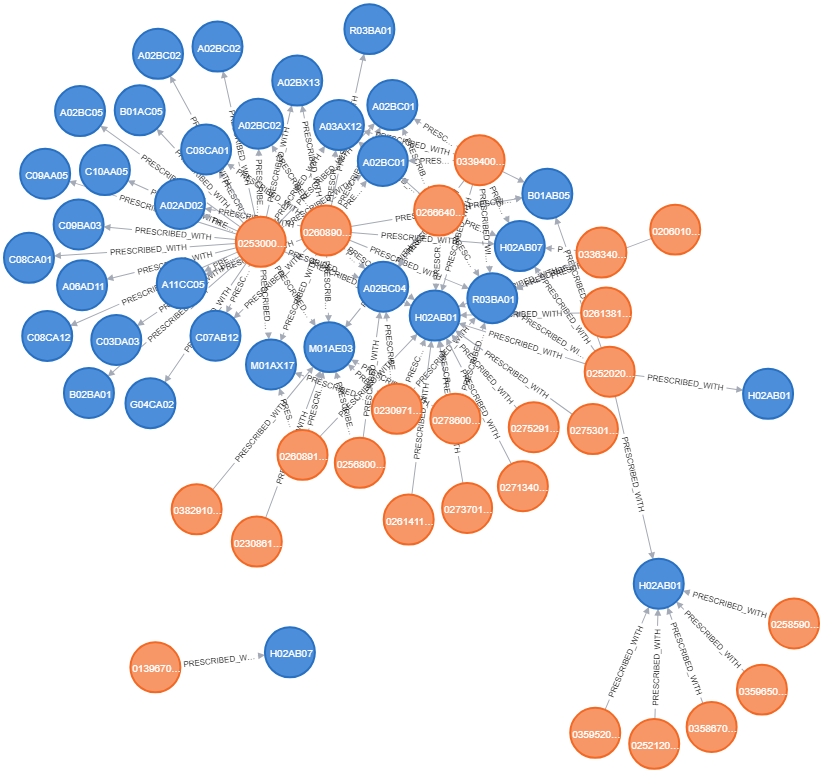
\includegraphics[scale=0.4]{./images/couples-graph.png}
	\caption{\small Co-prescriptions graph}
\end{figure}

Visualising the newly created relationships, two connected components are highlighted in figure 7.5 (orange antibiotics, blue other medicines).

\newpage
The component with only one couple corresponds to Plaquenil - Deltacortene, prescribed together approximately 5 000 times. Plaquenil can be used as antibiotic (antimalarial), but it is mostly given to treat arthritis, while Deltacortene is a corticosteroid for rheumatisms. 

The range of values varies from 4 145 to 38 153 in the timespan of 10 years. The 5 most popular co-prescriptions are:
\begin{enumerate}
	\item Augmentin - Oki;
	\item Rocefin - Bentelan;
	\item Augmentin - Bentelan;
	\item Normix - Cardioaspirin;
	\item Augmentin - Aulin.
\end{enumerate}

Bentelan is a corticosteroid which cannot be used without an antibiotic in presence of systemic (concerning the whole organism) infections, since it is an immunosuppressive drug, and this would explain the frequent co-prescriptions.

All the \textbf{antibiotics} are among the most prescribed ones, which justifies their presence in the co-prescriptions as well.

\subsection{Projecting prescriptive habits}
Having a detailed view of doctors' most common prescriptions gives another insight on how antibiotics are related.

\begin{figure}[h]
	\centering
	\includegraphics[scale=0.09]{./images/doctors-antibiotics-graph.png}
	\caption{\small Most prescribed antibiotics graph}
\end{figure}

The three most prescribed antibiotics for each doctor are taken, along with their count, and a new relationship OFTEN\_PRESCRIBED between Doctor and Antibiotic is created. Only amounts of prescriptions greater or equal to 50 are taken into account, for consistency of results, resulting in 2 353 links.

The obtained graph displays:
\begin{enumerate}
	\item 809 doctors, the light blue nodes;
	\item 95 antibiotics, the orange nodes.
\end{enumerate}

There are a few antibiotics in the centre (Augmentin and Normix), linked to a large amount of doctors, and external antibiotic nodes having rare prevalence.

Comparing the quantity of antibiotics and doctors and their relationships, it can be seen that most doctors prescribe a very restricted set of antibiotics. 

To have a better understanding of the popularity of specific drugs, an auxiliary relationship PRESCRIBED\_BY\_SAME\_DOCTOR is created between Antibiotics. 

\newpage
Antibiotics are interlinked with new relationships:

\begin{figure}[h]
	\centering
	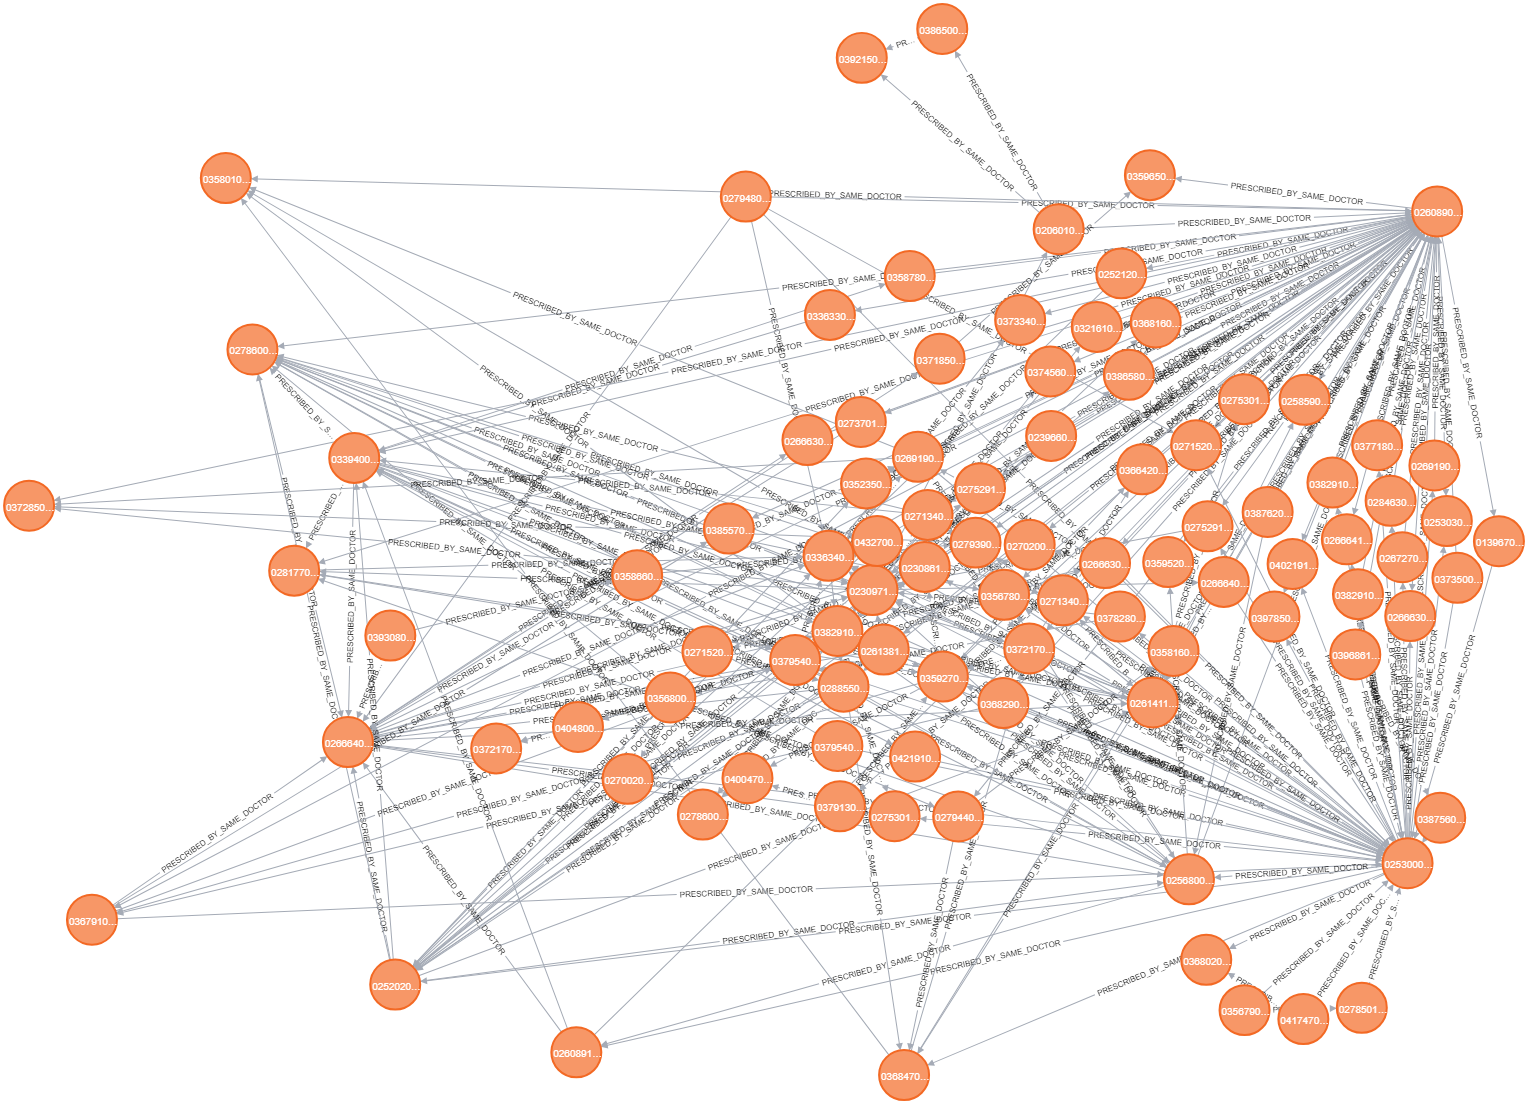
\includegraphics[scale=0.3]{./images/antibiotics-graph.png}
	\caption{\small Antibiotics prescribed by same doctors}
\end{figure}

95 nodes are connected by 294 relationships.

The previous graph confirms the discrepancy between popularity of antibiotics. Nodes on the top left have a higher number of connections, while ones on the bottom right tend to have fewer prescriptions.

One hypothesis consists in having a subset of common antibiotics shared between most general practitioners, and another one of individual preferences.

\section{Graph algorithms}
The final part of this research consists in wrapping up existing results and compare them to the ones obtained with a different methodology, applying graph algorithms.

\textbf{Graph algorithms} are the powerhouse behind analytics for connected systems. These algorithms use the connections between data to evaluate and infer the organization and dynamics of real-world systems\footnote{\href{https://neo4j.com/docs/pdf/neo4j-graph-algorithms-3.5.pdf}{Neo4j official documentation}}.

\subsection{Centrality algorithms}

\subsubsection{Betweenness}
The Betweenness Centrality algorithm calculates the shortest (weighted) path between every pair of nodes in a connected graph, using the breadth-first search algorithm. 

Each node receives a score, based on the number of these shortest paths that pass through the node. Nodes that most frequently lie on these shortest paths will have a higher betweenness centrality score. 

Betweenness among the top 5 \textbf{antibiotics}:
\begin{table}[h]
	\centering
	\begin{tabular}{c|c}
		\textbf{Antibiotic} & \textbf{Betweenness} \\
		\hline
		Augmentin (tablets) & 2 562 \\
		\hline
		Normix & 1 852,74 \\
		\hline
		Velamox & 683,78 \\
		\hline
		Ciproxin & 562,71 \\
		\hline
		Augmentin (bottles) & 489,93 \\
	\end{tabular}
\caption{\small Betweenness statistics for antibiotics}
\end{table}

As expected, the \textit{most prescribed} antibiotics have the highest betweenness scores: since they often get prescribed, the number of relationships involving the nodes is high, increasing the probability of a shortest path crossing them.

\subsubsection{Degree}
Degree Centrality is the simplest of all the centrality algorithms. It measures the number of incoming and outgoing relationships from a node, analysing its influence.

Degree among the top 5 \textit{antibiotics}, according to co-prescriptions:
\begin{table}[h]
	\centering
	\begin{tabular}{c|c}
		\textbf{Antibiotic} & \textbf{Degree} \\
		\hline
		Augmentin (tablets) & 32 \\
		\hline
		Normix & 22 \\
		\hline
		Ciproxin & 14 \\
		\hline
		Augmentin (bottles) & 12 \\
		\hline
		Velamox & 10 \\
	\end{tabular}
\caption{\small Degree statistics for antibiotics}
\end{table}

Results are similar to Betweenness Centrality, as expected: most prescribed products have the largest number of paths.

Another approach of Degree Centrality analysis involves general practitioners, to understand their influence as prescribers.

Calculating degree among \textbf{doctors} is useful to determine whether the top antibiotics prescribers are also the top prescribers, using the top 5 doctors.

\begin{table}[h]
	\centering
	\begin{tabular}{c|c|c|c|c}
		\textbf{Doctor} & \textbf{Degree (antibiotics)} & \textbf{Degree (medicine)} & \textbf{Total degree} & \textbf{Patients} \\
		\hline
		1 & 45 625 & 51 221 & 96 846 & 4 466 \\
		\hline
		2 & 42 554 & 41 594 & 84 148 & 2 022 \\
		\hline
		3 & 35 645 & 22 383 & 58 028 & 1 816 \\
		\hline
		4 & 34 587 & 40 315 & 74 902 & 2 028 \\
		\hline
		5 & 34 380 & 28 763 & 63 143 & 1 874
	\end{tabular}
\caption{\small Degree statistics for doctors}
\end{table}

Seeing the obtained results, the overprescribing of some general practitioners is clear: most of them makes a number of antibiotic prescriptions equal to others having double the amount of patients.

Doctors prescribing too much and not strictly when needed is one of the main causes of antibiotic resistance in Italy, therefore further analysis is required to assess changes in patients numbers and break down results in shorter time spans.

\subsection{Graph sampling}
Machine learning algorithms need a heavy amount of resources and computational time, therefore running clustering on a graph with nodes in the magnitude order of millions is not the best practice to extract insightful information in limited time.

Imposing small time ranges and only relevant features (lower bound on prescriptions) improves not only machine usage, but also accuracy of data. 

A new subset is extracted, selecting all data from the year 2017 of patients having arbitrarily at least \textbf{10 antibiotic prescriptions} during that year.

The new database is composed by:
\begin{itemize}
	\item 8 228 patients;
	\item 115 443 antibiotic prescriptions;
	\item 775 doctors;
	\item 946 antibiotics;
	\item 181 016 other prescriptions;
	\item 4 654 other medicines.
\end{itemize}

Having a time range of one year and only considering patients getting antibiotic prescriptions rather often does not offer additional information on antibiotic resistance, yet it allows to obtain relevant patterns of prescribing habits.

The output of graph processing will be used to apply computationally expensive graph algorithms. 

\subsection{Similarity detection}
Jaccard similarity is computed among \textbf{doctors}, considering the Cartesian product of nodes (775 $\times$ 775) with a threshold of 0.4 as coefficient. The result consists in about 500 values, which show the presence of clusters. The considered parameter to determine similarity is antibiotic prescribing (relationship between doctors and antibiotics), therefore linked nodes have the same habits.

The algorithm computes for each node, the most similar other node, according to the maximum Jaccard coefficient.

Doctors are then assigned a link, connecting similar pairs. Since a single doctor can be the most similar to several ones, nodes tend to group in clusters: connected components have a high probability of having common prescription patterns. 

\begin{figure}[h]
	\centering
	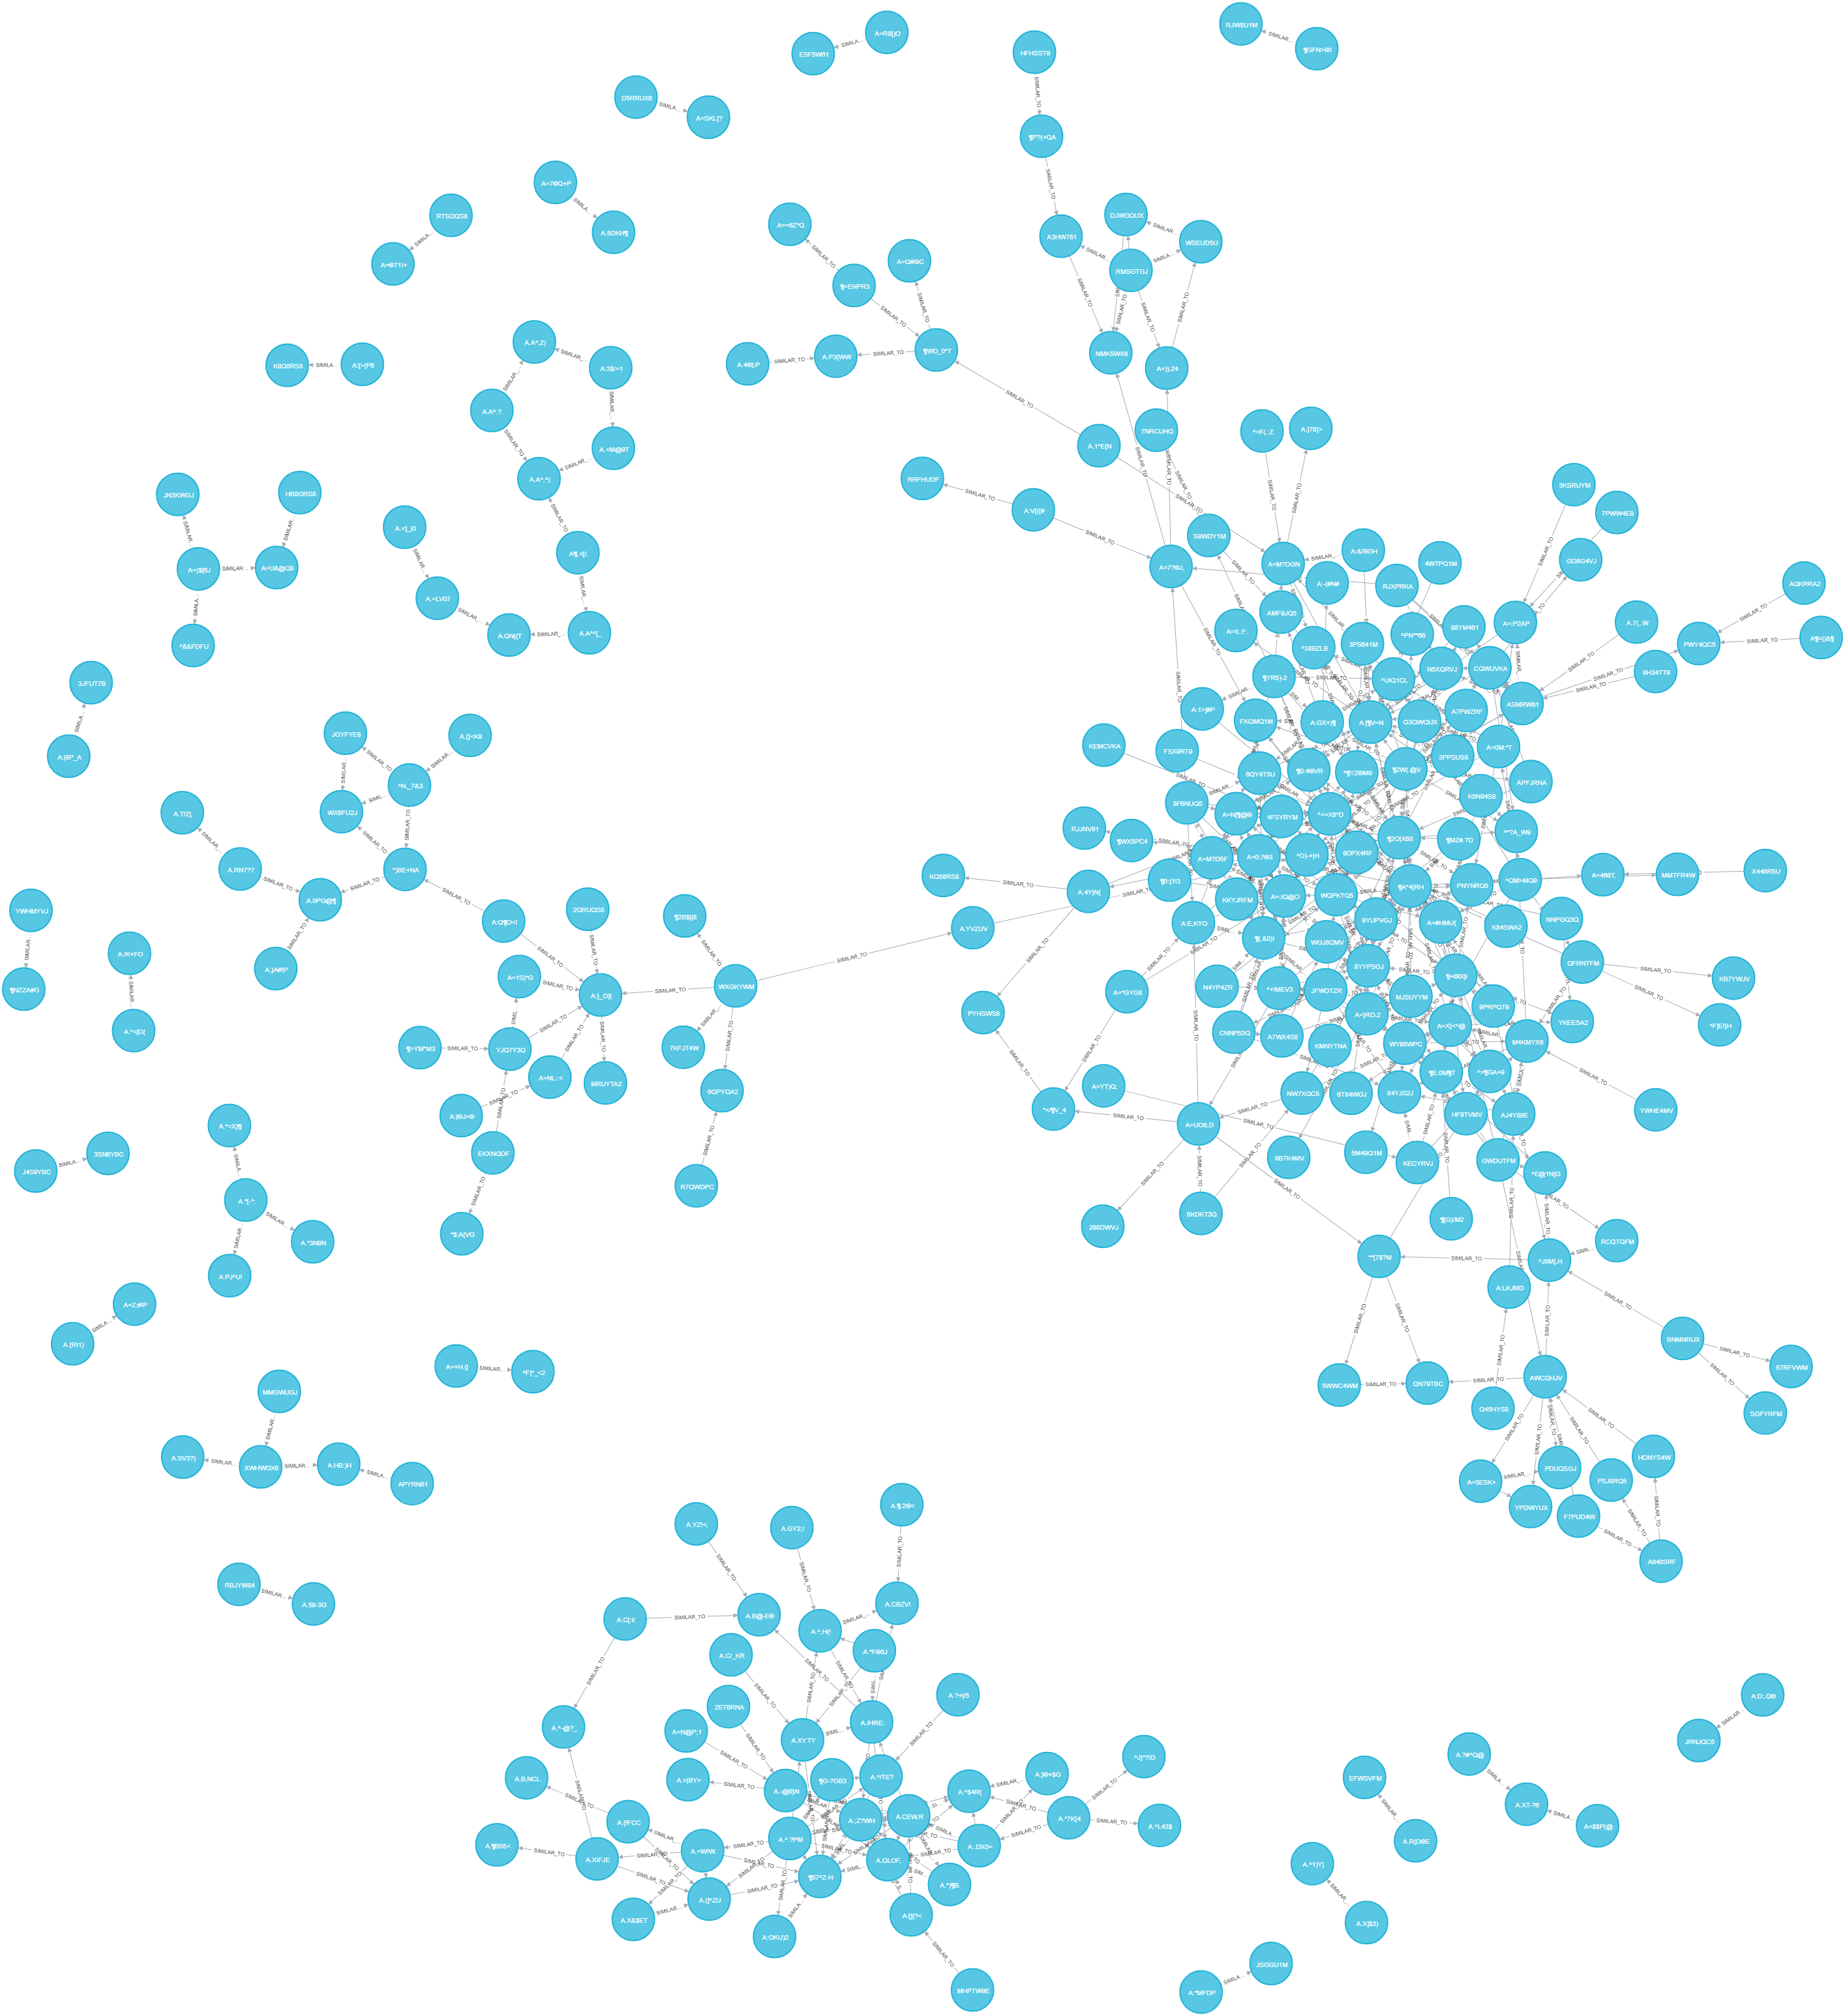
\includegraphics[scale=0.15]{./images/similarity-doctors.png}
	\caption{\small Similarity on doctors}
\end{figure}

A large cluster on the right (figure 7.8) groups most of general practitioners, confirming the hypothesis of popular antibiotics prescribed by the majority of individuals.

Going into a higher level of detail, Augmentin and Normix are the most common prescriptions, yet a single doctor \textit{often leans towards one} of the two instead of giving them both to patients. 

There also is a pair of doctors connecting different components of the graph, acting as a ``bridge'' between prescribers of different antibiotics.

\subsection{Community detection}
The concept of community refers to the structure (topological and relational aspects) of dense sub-components of a graph. Node attributes are considered as well, to obtain additional inferences on their membership. Data is linked with discrete attributes, and applications are based on graphs properties.

Identifying communities allows to understand the global functioning and relationships between individuals with the same features. Different groups interact between one another, and can be related, giving information on the global schema.

\begin{figure}[h]
	\centering
	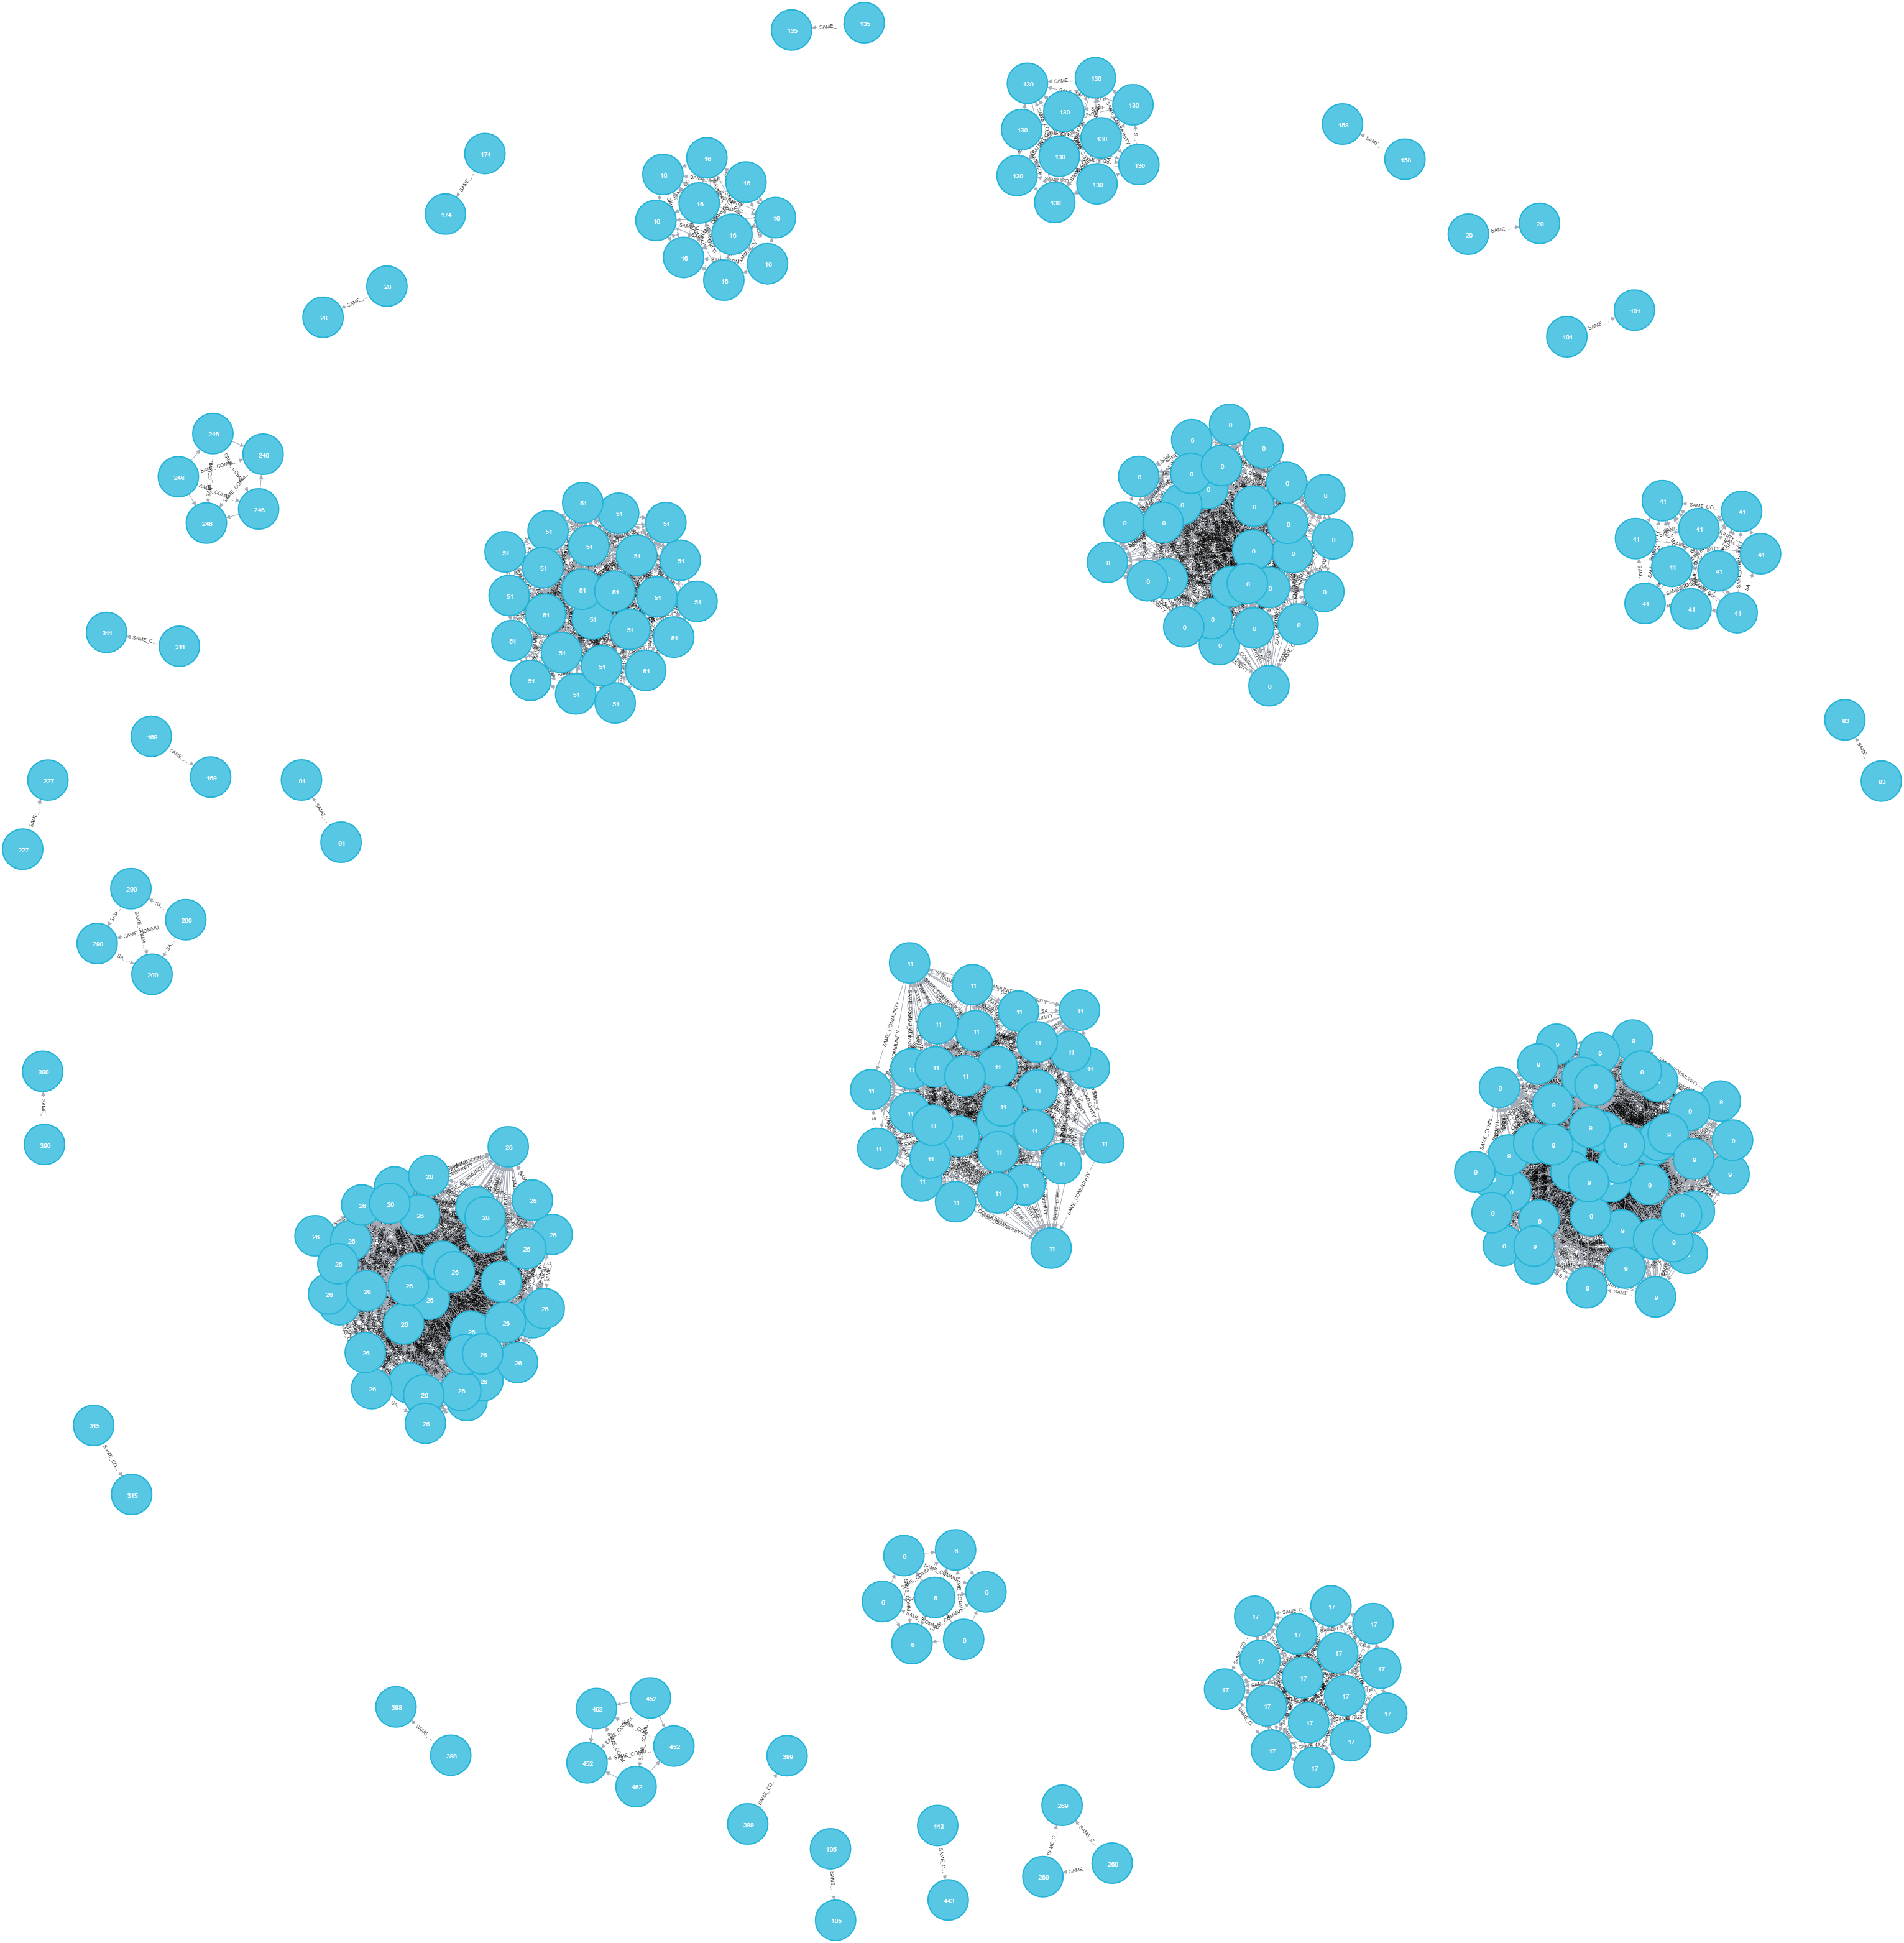
\includegraphics[scale=0.11]{./images/community-doctors.png}
	\caption{\small Communities of doctors}
\end{figure}

Communities are identified between \textbf{doctors} according to their similarity, based on antibiotic prescriptions and resulting in 526 communities, 495 of which are composed by a singlet. The presence of clusters implies that groups of doctors have the same prescriptive habits, while others do not fall in any specific category.

Results are similar to the $k$-means approach, although the considered dataset is significantly smaller: each community is distinguished by relevant characteristics, taking into account additional factors such as the amount of different products.

The first 5 communities in terms of numerosity are:
\begin{table}[h]
	\centering
	\begin{tabular}{c|c|c}
		\textbf{Community} & \textbf{Doctors}  & \textbf{Characteristic} \\
		\hline
		9 & 48 & Large Normix prescriptions \\
		\hline
		26 & 41 & Rare prescribers \\
		\hline
		11 & 31 & All antibiotics prescribers, large amount \\
		\hline
		0 $\cup$ 51 & 30 + 25 & All antibiotics prescribers, medium amount \\
		\hline
		17 & 16 & Large Augmentin prescribers \\
		\hline
	\end{tabular}
\caption{\small Communities statistics}
\end{table}

As expected, Normix and Augmentin prescribers are different classes of doctors: since both antibiotics are wide spectrum, the preference is most likely influenced by promotional factors or personal bias.

\section{Considerations}
Graph databases offer a completely different perspective compared to relational ones, allowing to understand behaviour of nodes and linkage between them.

Despite not having a relationship between each pair of node, the whole graph can be efficiently crossed through \textbf{paths}, displaying different views focussed on nodes or their type while linking them to the whole structure. 

Building targeted datasets and extracting features is immediate, adding relationships with eventual weight and filtering according to properties.

Those datasets or query results are fed to graph algorithms, which automatically stream or add resulting properties to then make further considerations without having to export data in a format readable by programming languages.

The main issue is encountered while \textit{handling large amount of data}: performance with ~200k nodes is optimal, yet scaling in the order of millions makes computationally expensive algorithms impossible to run in an acceptable amount of time.

Results are consistent with other machine learning approaches and exploration analytics, providing different methodologies to improve speed and comprehension.

Concrete outcomes after an approach with graphs consist in a further confirmation of the issue of antibiotic resistance, comparing doctors' degree to their number of patients and analyzing their prescriptive habits which, although clear, are concerning.

Co-prescriptions also highlight a major prevalence of a smaller set of products, influenced by the pressure of pharmaceutical companies and majorly prescribed for common diseases. 

